\documentclass[a4]{article}


\usepackage{epsfig}
\usepackage{amsfonts}
\usepackage{amssymb}
\usepackage{mathrsfs}
\usepackage{theorem}
\usepackage{amsmath}
\usepackage{times}
\usepackage{color}
\usepackage[french]{babel}
\usepackage[T1]{fontenc}
\usepackage{ifpdf}
\usepackage{epstopdf}   
\usepackage{url}


\begin{document}
\section{Toto}
Blabla
\begin{center}


\begin{figure*}[ht]
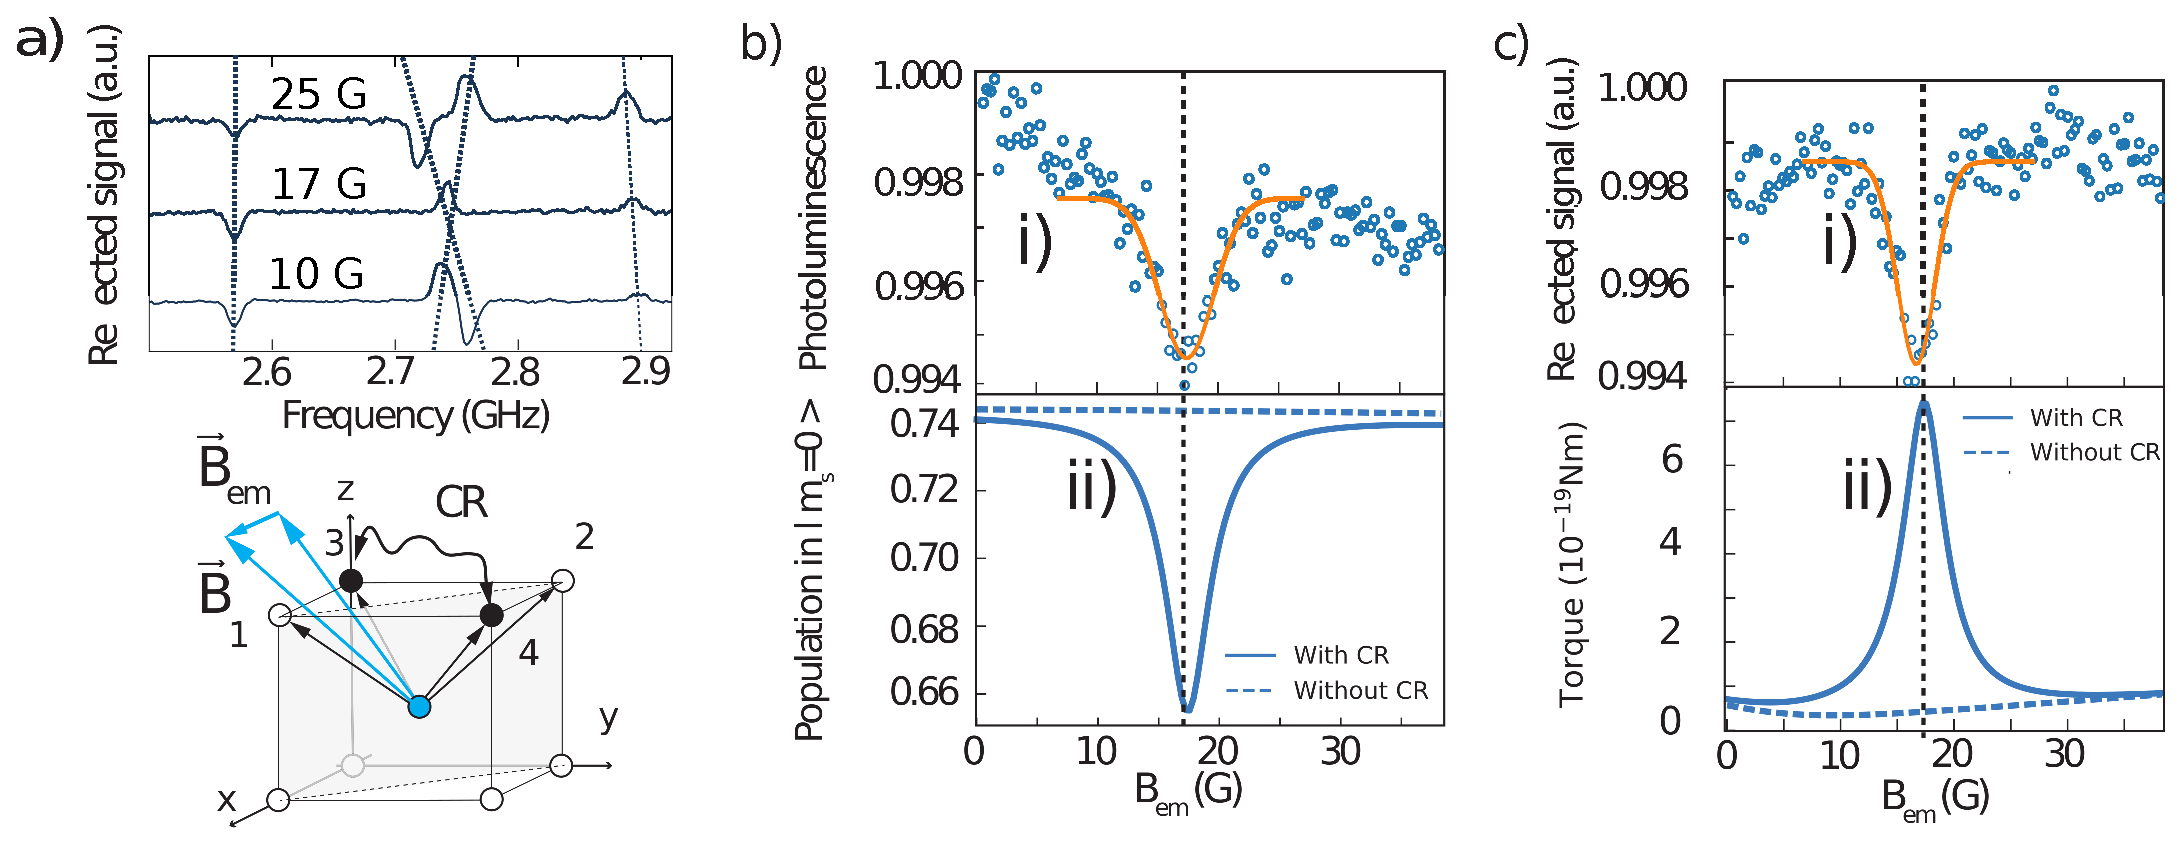
\includegraphics[scale=.6]{CRmeca}
\caption{ i) ESR spectra while scanning B$_{em}$ with some bias field applied. ii)Angular position of the diamond while scanning B$_{em}$ without a microwave. The rotation of the diamond at 17 G corresponds to the resonance between two classes of NV}

\end{figure*}
\end{center}
\end{document}